\PassOptionsToPackage{unicode=true}{hyperref} % options for packages loaded elsewhere
\PassOptionsToPackage{hyphens}{url}
\PassOptionsToPackage{dvipsnames,svgnames*,x11names*}{xcolor}
%
\documentclass[12pt,]{krantz}
\usepackage{lmodern}
\usepackage{amssymb,amsmath}
\usepackage{ifxetex,ifluatex}
\usepackage{fixltx2e} % provides \textsubscript
\ifnum 0\ifxetex 1\fi\ifluatex 1\fi=0 % if pdftex
  \usepackage[T1]{fontenc}
  \usepackage[utf8]{inputenc}
  \usepackage{textcomp} % provides euro and other symbols
\else % if luatex or xelatex
  \usepackage{unicode-math}
  \defaultfontfeatures{Ligatures=TeX,Scale=MatchLowercase}
\fi
% use upquote if available, for straight quotes in verbatim environments
\IfFileExists{upquote.sty}{\usepackage{upquote}}{}
% use microtype if available
\IfFileExists{microtype.sty}{%
\usepackage[]{microtype}
\UseMicrotypeSet[protrusion]{basicmath} % disable protrusion for tt fonts
}{}
\IfFileExists{parskip.sty}{%
\usepackage{parskip}
}{% else
\setlength{\parindent}{0pt}
\setlength{\parskip}{6pt plus 2pt minus 1pt}
}
\usepackage{xcolor}
\usepackage{hyperref}
\hypersetup{
            pdfauthor={Department of Psychology, The University of Edinburgh},
            colorlinks=true,
            linkcolor=Maroon,
            filecolor=Maroon,
            citecolor=Blue,
            urlcolor=Blue,
            breaklinks=true}
\urlstyle{same}  % don't use monospace font for urls
\usepackage{color}
\usepackage{fancyvrb}
\newcommand{\VerbBar}{|}
\newcommand{\VERB}{\Verb[commandchars=\\\{\}]}
\DefineVerbatimEnvironment{Highlighting}{Verbatim}{commandchars=\\\{\}}
% Add ',fontsize=\small' for more characters per line
\usepackage{framed}
\definecolor{shadecolor}{RGB}{248,248,248}
\newenvironment{Shaded}{\begin{snugshade}}{\end{snugshade}}
\newcommand{\AlertTok}[1]{\textcolor[rgb]{0.94,0.16,0.16}{#1}}
\newcommand{\AnnotationTok}[1]{\textcolor[rgb]{0.56,0.35,0.01}{\textbf{\textit{#1}}}}
\newcommand{\AttributeTok}[1]{\textcolor[rgb]{0.77,0.63,0.00}{#1}}
\newcommand{\BaseNTok}[1]{\textcolor[rgb]{0.00,0.00,0.81}{#1}}
\newcommand{\BuiltInTok}[1]{#1}
\newcommand{\CharTok}[1]{\textcolor[rgb]{0.31,0.60,0.02}{#1}}
\newcommand{\CommentTok}[1]{\textcolor[rgb]{0.56,0.35,0.01}{\textit{#1}}}
\newcommand{\CommentVarTok}[1]{\textcolor[rgb]{0.56,0.35,0.01}{\textbf{\textit{#1}}}}
\newcommand{\ConstantTok}[1]{\textcolor[rgb]{0.00,0.00,0.00}{#1}}
\newcommand{\ControlFlowTok}[1]{\textcolor[rgb]{0.13,0.29,0.53}{\textbf{#1}}}
\newcommand{\DataTypeTok}[1]{\textcolor[rgb]{0.13,0.29,0.53}{#1}}
\newcommand{\DecValTok}[1]{\textcolor[rgb]{0.00,0.00,0.81}{#1}}
\newcommand{\DocumentationTok}[1]{\textcolor[rgb]{0.56,0.35,0.01}{\textbf{\textit{#1}}}}
\newcommand{\ErrorTok}[1]{\textcolor[rgb]{0.64,0.00,0.00}{\textbf{#1}}}
\newcommand{\ExtensionTok}[1]{#1}
\newcommand{\FloatTok}[1]{\textcolor[rgb]{0.00,0.00,0.81}{#1}}
\newcommand{\FunctionTok}[1]{\textcolor[rgb]{0.00,0.00,0.00}{#1}}
\newcommand{\ImportTok}[1]{#1}
\newcommand{\InformationTok}[1]{\textcolor[rgb]{0.56,0.35,0.01}{\textbf{\textit{#1}}}}
\newcommand{\KeywordTok}[1]{\textcolor[rgb]{0.13,0.29,0.53}{\textbf{#1}}}
\newcommand{\NormalTok}[1]{#1}
\newcommand{\OperatorTok}[1]{\textcolor[rgb]{0.81,0.36,0.00}{\textbf{#1}}}
\newcommand{\OtherTok}[1]{\textcolor[rgb]{0.56,0.35,0.01}{#1}}
\newcommand{\PreprocessorTok}[1]{\textcolor[rgb]{0.56,0.35,0.01}{\textit{#1}}}
\newcommand{\RegionMarkerTok}[1]{#1}
\newcommand{\SpecialCharTok}[1]{\textcolor[rgb]{0.00,0.00,0.00}{#1}}
\newcommand{\SpecialStringTok}[1]{\textcolor[rgb]{0.31,0.60,0.02}{#1}}
\newcommand{\StringTok}[1]{\textcolor[rgb]{0.31,0.60,0.02}{#1}}
\newcommand{\VariableTok}[1]{\textcolor[rgb]{0.00,0.00,0.00}{#1}}
\newcommand{\VerbatimStringTok}[1]{\textcolor[rgb]{0.31,0.60,0.02}{#1}}
\newcommand{\WarningTok}[1]{\textcolor[rgb]{0.56,0.35,0.01}{\textbf{\textit{#1}}}}
\usepackage{longtable,booktabs}
% Fix footnotes in tables (requires footnote package)
\IfFileExists{footnote.sty}{\usepackage{footnote}\makesavenoteenv{longtable}}{}
\usepackage{graphicx,grffile}
\makeatletter
\def\maxwidth{\ifdim\Gin@nat@width>\linewidth\linewidth\else\Gin@nat@width\fi}
\def\maxheight{\ifdim\Gin@nat@height>\textheight\textheight\else\Gin@nat@height\fi}
\makeatother
% Scale images if necessary, so that they will not overflow the page
% margins by default, and it is still possible to overwrite the defaults
% using explicit options in \includegraphics[width, height, ...]{}
\setkeys{Gin}{width=\maxwidth,height=\maxheight,keepaspectratio}
\setlength{\emergencystretch}{3em}  % prevent overfull lines
\providecommand{\tightlist}{%
  \setlength{\itemsep}{0pt}\setlength{\parskip}{0pt}}
\setcounter{secnumdepth}{5}
% Redefines (sub)paragraphs to behave more like sections
\ifx\paragraph\undefined\else
\let\oldparagraph\paragraph
\renewcommand{\paragraph}[1]{\oldparagraph{#1}\mbox{}}
\fi
\ifx\subparagraph\undefined\else
\let\oldsubparagraph\subparagraph
\renewcommand{\subparagraph}[1]{\oldsubparagraph{#1}\mbox{}}
\fi

% set default figure placement to htbp
\makeatletter
\def\fps@figure{htbp}
\makeatother

\usepackage{booktabs}
\usepackage{amsthm}
\makeatletter
\def\thm@space@setup{%
  \thm@preskip=8pt plus 2pt minus 4pt
  \thm@postskip=\thm@preskip
}
\makeatother
\usepackage[]{natbib}
\bibliographystyle{apalike}

\title{Data Analysis for Psychology in R 1}
\author{Department of Psychology, The University of Edinburgh}
\date{Academic year 2020-2021}

\begin{document}
\maketitle

{
\hypersetup{linkcolor=}
\setcounter{tocdepth}{2}
\tableofcontents
}
\listoftables
\listoffigures
\hypertarget{chap-overview}{%
\section*{Course overview}\label{chap-overview}}
\addcontentsline{toc}{section}{Course overview}

\hypertarget{course-description}{%
\subsection*{Course description}\label{course-description}}
\addcontentsline{toc}{subsection}{Course description}

Data analysis for psychology in R 1 or, in short, \textbf{DAPR1}, is your first step on the exciting road of analysing data, and using data to answer interesting questions in the ways that statisticians, researchers, data scientists do.

This year-long course is designed to work gently through conceptual content that form the basis of understanding and working with data to perform statistical testing. It will provide you with the foundations in working with data and probability theory, and build to learning about how we make inferences about our hypotheses in psychology. Concepts are demonstrated in R throughout, taking you from basic calculations to the foundations of data management, plotting and use of simple statistical tests.

The overall aim of the course is to provide you with all the necessary skills to feel confident in the basics of statistics, R and data, before we move on to discuss a broader array of statistical methods in year 2.

\hypertarget{team}{%
\subsection*{Team}\label{team}}
\addcontentsline{toc}{subsection}{Team}

\begin{itemize}
\tightlist
\item
  Dr Tom Booth, \emph{Senior Lecturer}: \href{mailto:Tom.Booth@ed.ac.uk}{\nolinkurl{Tom.Booth@ed.ac.uk}}
\item
  Dr Josiah King, \emph{Senior Teaching Coordinator}: \href{mailto:ug.ppls.stats@ed.ac.uk}{\nolinkurl{ug.ppls.stats@ed.ac.uk}}
\item
  Dr Umberto Noe, \emph{Senior Teaching Coordinator}: \href{mailto:ug.ppls.stats@ed.ac.uk}{\nolinkurl{ug.ppls.stats@ed.ac.uk}}
\item
  And not forgetting your friendly tutoring team! Ask them anything!
\end{itemize}

\hypertarget{schedule}{%
\subsection*{Schedule}\label{schedule}}
\addcontentsline{toc}{subsection}{Schedule}

\textbf{SEMESTER 1}

\begin{longtable}[]{@{}ll@{}}
\toprule
Week & Topic\tabularnewline
\midrule
\endhead
1 & Collecting data\tabularnewline
2 & Types of data\tabularnewline
3 & Visualising distributions\tabularnewline
4 & Describing distributions\tabularnewline
5 & Visualising and describing relationships\tabularnewline
Break &\tabularnewline
6 & Basics of probability theory\tabularnewline
7 & Probability rules\tabularnewline
8 & Random variables\tabularnewline
9 & Sampling variability and sampling distributions\tabularnewline
10 & Bias-variance trade-off\tabularnewline
\bottomrule
\end{longtable}

\textbf{SEMESTER 2}

\begin{longtable}[]{@{}ll@{}}
\toprule
Week & Topic\tabularnewline
\midrule
\endhead
11 & Bootstrap \& Confidence Intervals\tabularnewline
12 & Hypothesis testing with the p-value approach\tabularnewline
13 & Hypothesis testing with the critical values approach\tabularnewline
14 & Hypothesis testing \& Confidence Intervals\tabularnewline
15 & Making decisions - Effect sizes, Power, Errors\tabularnewline
Break &\tabularnewline
16 & Test for one mean\tabularnewline
17 & Test for two means (paired samples)\tabularnewline
18 & Test for two means (independent samples)\tabularnewline
19 & Chi-square test\tabularnewline
20 & Covariance, correlation, and looking ahead\tabularnewline
\bottomrule
\end{longtable}

\hypertarget{textbook}{%
\subsection*{Textbook}\label{textbook}}
\addcontentsline{toc}{subsection}{Textbook}

TBC

\hypertarget{chap-collecting-data}{%
\section{Collecting Data}\label{chap-collecting-data}}

\hypertarget{learning-objectives}{%
\subsection*{Learning Objectives}\label{learning-objectives}}
\addcontentsline{toc}{subsection}{Learning Objectives}

\begin{itemize}
\tightlist
\item
  LO1: Install R \& Rstudio, and get comfortable with the layout\\
\item
  LO2: Learn about how data is stored in R
\item
  LO3: Produce your first Rmarkdown document\\
\end{itemize}

\hypertarget{r-rstudio}{%
\subsection*{R \& Rstudio}\label{r-rstudio}}
\addcontentsline{toc}{subsection}{R \& Rstudio}

\hypertarget{installing-r-rstudio}{%
\subsubsection*{Installing R \& Rstudio}\label{installing-r-rstudio}}
\addcontentsline{toc}{subsubsection}{Installing R \& Rstudio}

install tidyverse, rmarkdown, knitr etc.

\hypertarget{intro-to-rstudio}{%
\subsubsection*{Intro to Rstudio}\label{intro-to-rstudio}}
\addcontentsline{toc}{subsubsection}{Intro to Rstudio}

useful settings -
environment clearing
soft-wrapping text

\hypertarget{r-as-a-calculator}{%
\subsubsection*{R as a calculator}\label{r-as-a-calculator}}
\addcontentsline{toc}{subsubsection}{R as a calculator}

\hypertarget{rscripts-rmarkdown}{%
\subsubsection*{Rscripts, Rmarkdown}\label{rscripts-rmarkdown}}
\addcontentsline{toc}{subsubsection}{Rscripts, Rmarkdown}

\hypertarget{using-r-packages}{%
\subsubsection*{Using R packages}\label{using-r-packages}}
\addcontentsline{toc}{subsubsection}{Using R packages}

\hypertarget{data-in-r}{%
\subsection*{Data in R}\label{data-in-r}}
\addcontentsline{toc}{subsection}{Data in R}

assignment \texttt{\textless{}-}
vector
matrix
data.frame
tibble

accessors {[}{]}, \$

\hypertarget{tasks-for-today}{%
\subsection*{Tasks for today}\label{tasks-for-today}}
\addcontentsline{toc}{subsection}{Tasks for today}

\textbf{Task}
Open an Rmarkdown document.

\textbf{File \textgreater{} New File \textgreater{} R Markdown..}

When the box pops-up, give a title of your choice (``Intro lab'', maybe?) and your name as the author.

The file which opens will have some template stuff in it. Delete everything below the first code chunk to start with a fresh document:

TODO IMAGE

\textbf{Task}
Insert a new code chunk by either using the Insert button in the top right of the document, and clicking R, or typing \emph{Ctrl + Alt + i}

Inside the chunk, type:\\
\texttt{print("Hello\ world!\ My\ name\ is\ ?")}.\\
Run the chunk and see that the output will be printed below.

\textbf{Task}
We're going to use some functions which are in the \textbf{tidverse} package, which we have already installed earlier on.\\
However, to \emph{use} the package, we need to load it using \texttt{library(tidyverse)}.

\textbf{Important:} When writing analysis, we want it to be \emph{reproducible}.\\
We want to be able to give somebody else our code and the data, and ensure that they can get the same results.
To do this, we need to show what packages we use.\\
It is good practice to load any packages you use at the top of your code.

In your first code chunk, type:

\begin{Shaded}
\begin{Highlighting}[]
\CommentTok{#I'm going to use these packages in this document:}
\KeywordTok{library}\NormalTok{(tidyverse)}
\end{Highlighting}
\end{Shaded}

and run the chunk.

Note that the \texttt{\#} in R code makes that line a comment, which basically means that R will ignore the line. Comments are useful for you to remind yourself of what your code is doing.

\textbf{Task}
\textbf{Below} the code chunk, add a new line with the following:

\texttt{\#\ R\ code\ examples}

When the \# is used in a Rmarkdown file, \textbf{outside} of a code-chunk, it makes that line a heading when we finally get to \emph{compiling} the document. Below, what you see on the left will be compiled to look like those on the right:

\begin{center}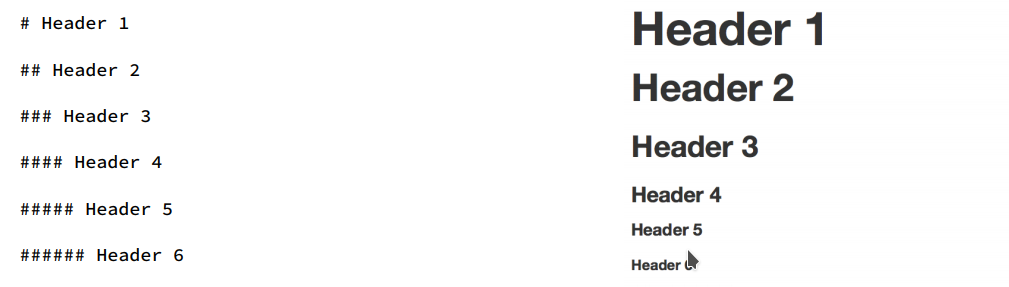
\includegraphics[width=0.4\linewidth]{images/headings} \end{center}

\textbf{Task}
In your Rmarkdown document, give an explanation of what each of the following does in R.
Write the explanation, and give an example in a code chunk.

\begin{itemize}
\tightlist
\item
  \texttt{+}
\item
  \texttt{-}
\item
  \texttt{*}
\item
  \texttt{/}
\item
  \texttt{()}
\item
  \texttt{\^{}}
\item
  \texttt{\textless{}-}
\item
  \texttt{=}
\item
  \texttt{\textless{}}
\item
  \texttt{\textgreater{}}
\item
  \texttt{\textless{}=}
\item
  \texttt{\textgreater{}=}
\item
  \texttt{==}
\item
  \texttt{!=}
\item
  \texttt{data.frame()}
\item
  \texttt{c()}
\item
  \texttt{{[}{]}}
\item
  \texttt{\$}
\end{itemize}

You can see an example of the first few below:
TODO IMAGE

\textbf{Solution }
Hopefully you managed to include examples for all of these, but we have provided a table below describing what each symbol does.

\begin{longtable}[]{@{}rrr@{}}
\toprule
\begin{minipage}[b]{0.30\columnwidth}\raggedleft
Symbol\strut
\end{minipage} & \begin{minipage}[b]{0.30\columnwidth}\raggedleft
Description\strut
\end{minipage} & \begin{minipage}[b]{0.30\columnwidth}\raggedleft
Example\strut
\end{minipage}\tabularnewline
\midrule
\endhead
\begin{minipage}[t]{0.30\columnwidth}\raggedleft
\texttt{+}\strut
\end{minipage} & \begin{minipage}[t]{0.30\columnwidth}\raggedleft
Adds two numbers together\strut
\end{minipage} & \begin{minipage}[t]{0.30\columnwidth}\raggedleft
\texttt{2+2} - two plus two\strut
\end{minipage}\tabularnewline
\begin{minipage}[t]{0.30\columnwidth}\raggedleft
\texttt{-}\strut
\end{minipage} & \begin{minipage}[t]{0.30\columnwidth}\raggedleft
Subtract one number from another\strut
\end{minipage} & \begin{minipage}[t]{0.30\columnwidth}\raggedleft
\texttt{3-1} - three minus one\strut
\end{minipage}\tabularnewline
\begin{minipage}[t]{0.30\columnwidth}\raggedleft
\texttt{*}\strut
\end{minipage} & \begin{minipage}[t]{0.30\columnwidth}\raggedleft
Multiply two numbers together\strut
\end{minipage} & \begin{minipage}[t]{0.30\columnwidth}\raggedleft
\texttt{3*3} - three times three\strut
\end{minipage}\tabularnewline
\begin{minipage}[t]{0.30\columnwidth}\raggedleft
\texttt{/}\strut
\end{minipage} & \begin{minipage}[t]{0.30\columnwidth}\raggedleft
Divide one number by another\strut
\end{minipage} & \begin{minipage}[t]{0.30\columnwidth}\raggedleft
\texttt{9/3} - nine divided by three\strut
\end{minipage}\tabularnewline
\begin{minipage}[t]{0.30\columnwidth}\raggedleft
\texttt{()}\strut
\end{minipage} & \begin{minipage}[t]{0.30\columnwidth}\raggedleft
group operations together\strut
\end{minipage} & \begin{minipage}[t]{0.30\columnwidth}\raggedleft
\texttt{(2+2)/4} is different from \texttt{2+2/4}\strut
\end{minipage}\tabularnewline
\begin{minipage}[t]{0.30\columnwidth}\raggedleft
\texttt{\^{}}\strut
\end{minipage} & \begin{minipage}[t]{0.30\columnwidth}\raggedleft
to the power of..\strut
\end{minipage} & \begin{minipage}[t]{0.30\columnwidth}\raggedleft
\texttt{4\^{}2} - four to the power of two, or four squared\strut
\end{minipage}\tabularnewline
\begin{minipage}[t]{0.30\columnwidth}\raggedleft
\texttt{\textless{}-}\strut
\end{minipage} & \begin{minipage}[t]{0.30\columnwidth}\raggedleft
stores an object in R with the left hand side (LHS) as the name, and the RHS as the value\strut
\end{minipage} & \begin{minipage}[t]{0.30\columnwidth}\raggedleft
\texttt{x\textless{}-10}\strut
\end{minipage}\tabularnewline
\begin{minipage}[t]{0.30\columnwidth}\raggedleft
\texttt{=}\strut
\end{minipage} & \begin{minipage}[t]{0.30\columnwidth}\raggedleft
stores an object in R with the left hand side (LHS) as the name, and the RHS as the value\strut
\end{minipage} & \begin{minipage}[t]{0.30\columnwidth}\raggedleft
\texttt{x\ =\ 10}\strut
\end{minipage}\tabularnewline
\begin{minipage}[t]{0.30\columnwidth}\raggedleft
\texttt{\textless{}}\strut
\end{minipage} & \begin{minipage}[t]{0.30\columnwidth}\raggedleft
is less than?\strut
\end{minipage} & \begin{minipage}[t]{0.30\columnwidth}\raggedleft
\texttt{2\textless{}3}\strut
\end{minipage}\tabularnewline
\begin{minipage}[t]{0.30\columnwidth}\raggedleft
\texttt{\textgreater{}}\strut
\end{minipage} & \begin{minipage}[t]{0.30\columnwidth}\raggedleft
is greater than?\strut
\end{minipage} & \begin{minipage}[t]{0.30\columnwidth}\raggedleft
\texttt{2\textgreater{}3}\strut
\end{minipage}\tabularnewline
\begin{minipage}[t]{0.30\columnwidth}\raggedleft
\texttt{\textless{}=}\strut
\end{minipage} & \begin{minipage}[t]{0.30\columnwidth}\raggedleft
is less than or equal to?\strut
\end{minipage} & \begin{minipage}[t]{0.30\columnwidth}\raggedleft
\texttt{2\textless{}=3}\strut
\end{minipage}\tabularnewline
\begin{minipage}[t]{0.30\columnwidth}\raggedleft
\texttt{\textgreater{}=}\strut
\end{minipage} & \begin{minipage}[t]{0.30\columnwidth}\raggedleft
is greater than or equal to?\strut
\end{minipage} & \begin{minipage}[t]{0.30\columnwidth}\raggedleft
\texttt{2\textgreater{}=2}\strut
\end{minipage}\tabularnewline
\begin{minipage}[t]{0.30\columnwidth}\raggedleft
\texttt{==}\strut
\end{minipage} & \begin{minipage}[t]{0.30\columnwidth}\raggedleft
is equal to?\strut
\end{minipage} & \begin{minipage}[t]{0.30\columnwidth}\raggedleft
\texttt{(5+5)\ ==\ 10}\strut
\end{minipage}\tabularnewline
\begin{minipage}[t]{0.30\columnwidth}\raggedleft
\texttt{!=}\strut
\end{minipage} & \begin{minipage}[t]{0.30\columnwidth}\raggedleft
is not equal to?\strut
\end{minipage} & \begin{minipage}[t]{0.30\columnwidth}\raggedleft
\texttt{(2+3)\ !=\ 4}\strut
\end{minipage}\tabularnewline
\begin{minipage}[t]{0.30\columnwidth}\raggedleft
\texttt{c()}\strut
\end{minipage} & \begin{minipage}[t]{0.30\columnwidth}\raggedleft
combines values into a vector (a sequence of values)\strut
\end{minipage} & \begin{minipage}[t]{0.30\columnwidth}\raggedleft
\texttt{c(1,2,3,4)}\strut
\end{minipage}\tabularnewline
\begin{minipage}[t]{0.30\columnwidth}\raggedleft
\texttt{data.frame()}\strut
\end{minipage} & \begin{minipage}[t]{0.30\columnwidth}\raggedleft
converts whatever is inside the brackets to a dataframe\strut
\end{minipage} & \begin{minipage}[t]{0.30\columnwidth}\raggedleft
\texttt{data.frame(values\ =\ c(1,2,3,4))}\strut
\end{minipage}\tabularnewline
\begin{minipage}[t]{0.30\columnwidth}\raggedleft
\texttt{{[}{]}}\strut
\end{minipage} & \begin{minipage}[t]{0.30\columnwidth}\raggedleft
used to extract the 1st, 2nd, \ldots{} \(i^{th}\) elements in a set of numbers\strut
\end{minipage} & \begin{minipage}[t]{0.30\columnwidth}\raggedleft
\texttt{myvector{[}3{]}}\strut
\end{minipage}\tabularnewline
\begin{minipage}[t]{0.30\columnwidth}\raggedleft
\texttt{\$}\strut
\end{minipage} & \begin{minipage}[t]{0.30\columnwidth}\raggedleft
used to extract a named column from a dataframe\strut
\end{minipage} & \begin{minipage}[t]{0.30\columnwidth}\raggedleft
\texttt{mydata\$age\_variable}\strut
\end{minipage}\tabularnewline
\bottomrule
\end{longtable}

\textbf{Task}
\textbf{Outside} of a code chunk, add a new heading with the following:

\texttt{\#\ Vectors\ and\ dataframes}

\textbf{Task}
In a new code chunk, do the following:

\begin{enumerate}
\def\labelenumi{\arabic{enumi}.}
\tightlist
\item
  store the following numbers as an object in R:\\
  4,7,3,1,8,9,5,2,2,6,9,9,5,20\\
\item
  Try using the function \texttt{sum()}, with the name of your object inside the brackets.
\end{enumerate}

\textbf{Solution }
Because this is just a set of numbers, we store it as a \textbf{vector}, using \texttt{c()}.\\
We have named it \texttt{myvec}, but you can call yours whatever you like.

The \texttt{sum()} function will add all of the numbers together!

\begin{Shaded}
\begin{Highlighting}[]
\NormalTok{myvec <-}\StringTok{ }\KeywordTok{c}\NormalTok{(}\DecValTok{4}\NormalTok{,}\DecValTok{7}\NormalTok{,}\DecValTok{3}\NormalTok{,}\DecValTok{1}\NormalTok{,}\DecValTok{8}\NormalTok{,}\DecValTok{9}\NormalTok{,}\DecValTok{5}\NormalTok{,}\DecValTok{2}\NormalTok{,}\DecValTok{2}\NormalTok{,}\DecValTok{6}\NormalTok{,}\DecValTok{9}\NormalTok{,}\DecValTok{9}\NormalTok{,}\DecValTok{5}\NormalTok{,}\DecValTok{20}\NormalTok{)}
\KeywordTok{sum}\NormalTok{(myvec)}
\end{Highlighting}
\end{Shaded}

\begin{verbatim}
[1] 90
\end{verbatim}

\textbf{Task}
Using the square brackets - \texttt{{[}{]}} - pull out the 2nd, 4th and 6th values in the object you just created.

\textbf{Hint:} You will need to put inside the square brackets a \emph{sequence of} numbers. How do we combine numbers in to a sequence in R? using \texttt{c()}!

\textbf{Solution }

\begin{Shaded}
\begin{Highlighting}[]
\NormalTok{myvec[}\KeywordTok{c}\NormalTok{(}\DecValTok{2}\NormalTok{,}\DecValTok{4}\NormalTok{,}\DecValTok{6}\NormalTok{)]}
\end{Highlighting}
\end{Shaded}

\begin{verbatim}
[1] 7 1 9
\end{verbatim}

\textbf{Task}
Store the names and birth-years of the Beatle in the appropriate format in R. Name it \texttt{beatles}.
John was born in 1940
Paul was born in 1942
George was born in 1943
Ringo was born in 1940

\textbf{Hint:} We're going to have two sequences here, the names, and the birth-years. The easiest way to think of this would be to have a row for each Beatle, and a column for each of name and birth-year.

Check dimensions of the object using \texttt{dim()}. How many rows and how many columns are there?

\textbf{Solution }
TODO - decide dataframe/tibble
We want a dataframe/tibble

\begin{Shaded}
\begin{Highlighting}[]
\NormalTok{beatles <-}\StringTok{ }
\StringTok{  }\KeywordTok{data.frame}\NormalTok{(}
    \DataTypeTok{name =} \KeywordTok{c}\NormalTok{(}\StringTok{"John"}\NormalTok{,}\StringTok{"Paul"}\NormalTok{,}\StringTok{"George"}\NormalTok{,}\StringTok{"Ringo"}\NormalTok{),}
    \DataTypeTok{birthyear =} \KeywordTok{c}\NormalTok{(}\DecValTok{1940}\NormalTok{,}\DecValTok{1942}\NormalTok{,}\DecValTok{1943}\NormalTok{,}\DecValTok{1940}\NormalTok{)}
\NormalTok{)}
\NormalTok{beatles <-}\StringTok{ }
\StringTok{  }\KeywordTok{tibble}\NormalTok{(}
    \DataTypeTok{name =} \KeywordTok{c}\NormalTok{(}\StringTok{"John"}\NormalTok{,}\StringTok{"Paul"}\NormalTok{,}\StringTok{"George"}\NormalTok{,}\StringTok{"Ringo"}\NormalTok{),}
    \DataTypeTok{birthyear =} \KeywordTok{c}\NormalTok{(}\DecValTok{1940}\NormalTok{,}\DecValTok{1942}\NormalTok{,}\DecValTok{1943}\NormalTok{,}\DecValTok{1940}\NormalTok{)}
\NormalTok{)}
\end{Highlighting}
\end{Shaded}

\begin{Shaded}
\begin{Highlighting}[]
\KeywordTok{dim}\NormalTok{(beatles)}
\end{Highlighting}
\end{Shaded}

\begin{verbatim}
[1] 4 2
\end{verbatim}

Four rows, and two columns!

\begin{center}\rule{0.5\linewidth}{0.5pt}\end{center}

So far, we've been manually inputting our data. However, R can read in data which has been created elsewhere (like in excel, or by some software which is used to present participants with experiments).

TODO - link to data we're going to use next couple of weeks

First, click on the following link: \href{https://uoe-psychology.github.io/uoe_psystats/multivar/data/women_computer_science.csv}{link}

It should open a webpage and show you a dataset.
There are two things to note.

\begin{itemize}
\tightlist
\item
  the values are separated by commas
\item
  the url (in the top bar of your browser) ends with \textbf{.csv}.
\end{itemize}

This stands for `comma separated value'.\\
The \textbf{tidyverse} package which we loaded at the top has a function to read this sort of data: \texttt{read\_csv()}.

\textbf{Task}
Read the data into R. You can do this by giving \texttt{read\_csv()} the url.

\textbf{Hint:} If you just type:

\begin{Shaded}
\begin{Highlighting}[]
\KeywordTok{read_csv}\NormalTok{(}\StringTok{"https://uoe-psychology.github.io/uoe_psystats/multivar/data/women_computer_science.csv"}\NormalTok{)}
\end{Highlighting}
\end{Shaded}

\begin{verbatim}
# A tibble: 192 x 3
    date field            pct_women_majors
   <dbl> <chr>                       <dbl>
 1  1966 Computer.science            0.146
 2  1967 Computer.science            0.108
 3  1968 Computer.science            0.12 
 4  1969 Computer.science            0.13 
 5  1970 Computer.science            0.129
 6  1971 Computer.science            0.136
 7  1972 Computer.science            0.136
 8  1973 Computer.science            0.149
 9  1974 Computer.science            0.164
10  1975 Computer.science            0.19 
# ... with 182 more rows
\end{verbatim}

It will print out the dataset, but it won't store it in R for you to do things with. To do that, we want to assign a name to the data:

\begin{Shaded}
\begin{Highlighting}[]
\NormalTok{mydata <-}\StringTok{ }\KeywordTok{read_csv}\NormalTok{(}\StringTok{"https://uoe-psychology.github.io/uoe_psystats/multivar/data/women_computer_science.csv"}\NormalTok{)}
\end{Highlighting}
\end{Shaded}

Note that it now turns up in the \emph{Environment} pane of Rstudio.

\textbf{Task}
Check how many rows and columns you have in the dataset.
You can do this with the \texttt{dim()} function.

\textbf{Solution }

\begin{Shaded}
\begin{Highlighting}[]
\KeywordTok{dim}\NormalTok{(mydata)}
\end{Highlighting}
\end{Shaded}

\begin{verbatim}
[1] 192   3
\end{verbatim}

\textbf{Task}
Using the square brackets, show the 167th row, with all columns.

\textbf{Remember:} When you are using \texttt{{[}{]}} with a dataframe, you specify \texttt{data{[}rows,\ columns{]}}. If you leave either rows or columns blank it will give all of them - for instance, \texttt{data{[}\ ,\ columns{]}} will give you all rows for some specified columns.

\textbf{Solution }

\begin{Shaded}
\begin{Highlighting}[]
\NormalTok{mydata[}\DecValTok{167}\NormalTok{,]}
\end{Highlighting}
\end{Shaded}

\begin{verbatim}
# A tibble: 1 x 3
   date field             pct_women_majors
  <dbl> <chr>                        <dbl>
1  1988 Physical.Sciences             0.32
\end{verbatim}

\begin{center}\rule{0.5\linewidth}{0.5pt}\end{center}

\textbf{Task}
By now, you should have an Rmardkown document ( \textbf{.Rmd} ) with your answers to the tasks we've been through today.

Compile the document by clicking on the \textbf{Knit} button at the top. The little arrow to the right allows you to compile to either \textbf{.pdf} or \textbf{.html}.

\hypertarget{glossary}{%
\subsection*{Glossary}\label{glossary}}
\addcontentsline{toc}{subsection}{Glossary}

\hypertarget{chap-data-types}{%
\section{Types of data}\label{chap-data-types}}

\hypertarget{learning-objectives-1}{%
\subsection*{Learning Objectives}\label{learning-objectives-1}}
\addcontentsline{toc}{subsection}{Learning Objectives}

\begin{itemize}
\tightlist
\item
  LO1:
\item
  LO2:
\item
  LO3:
\end{itemize}

\hypertarget{chap-visualising-distributions}{%
\section{Visualising distributions}\label{chap-visualising-distributions}}

\hypertarget{learning-objectives-2}{%
\subsection*{Learning Objectives}\label{learning-objectives-2}}
\addcontentsline{toc}{subsection}{Learning Objectives}

\begin{itemize}
\tightlist
\item
  LO1:
\item
  LO2:
\item
  LO3:
\end{itemize}

\hypertarget{chap-describing-distributions}{%
\section{Describing distributions}\label{chap-describing-distributions}}

\hypertarget{learning-objectives-3}{%
\subsection*{Learning Objectives}\label{learning-objectives-3}}
\addcontentsline{toc}{subsection}{Learning Objectives}

\begin{itemize}
\tightlist
\item
  LO1:
\item
  LO2:
\item
  LO3:
\end{itemize}

\hypertarget{chap-relationships}{%
\section{Visualising and describing relationships}\label{chap-relationships}}

\hypertarget{learning-objectives-4}{%
\subsection*{Learning Objectives}\label{learning-objectives-4}}
\addcontentsline{toc}{subsection}{Learning Objectives}

\begin{itemize}
\tightlist
\item
  LO1:
\item
  LO2:
\item
  LO3:
\end{itemize}

\hypertarget{chap-probability-theory}{%
\section{Basics of probability theory}\label{chap-probability-theory}}

\hypertarget{learning-objectives-5}{%
\subsection*{Learning Objectives}\label{learning-objectives-5}}
\addcontentsline{toc}{subsection}{Learning Objectives}

\begin{itemize}
\tightlist
\item
  LO1:
\item
  LO2:
\item
  LO3:
\end{itemize}

\hypertarget{chap-probability-rules}{%
\section{Probability rules}\label{chap-probability-rules}}

\hypertarget{learning-objectives-6}{%
\subsection*{Learning Objectives}\label{learning-objectives-6}}
\addcontentsline{toc}{subsection}{Learning Objectives}

\begin{itemize}
\tightlist
\item
  LO1:
\item
  LO2:
\item
  LO3:
\end{itemize}

\hypertarget{chap-random-variables}{%
\section{Random variables}\label{chap-random-variables}}

\hypertarget{learning-objectives-7}{%
\subsection*{Learning Objectives}\label{learning-objectives-7}}
\addcontentsline{toc}{subsection}{Learning Objectives}

\begin{itemize}
\tightlist
\item
  LO1:
\item
  LO2:
\item
  LO3:
\end{itemize}

\hypertarget{chap-sampling}{%
\section{Sampling variability and sampling distributions}\label{chap-sampling}}

\hypertarget{learning-objectives-8}{%
\subsection*{Learning Objectives}\label{learning-objectives-8}}
\addcontentsline{toc}{subsection}{Learning Objectives}

\begin{itemize}
\tightlist
\item
  LO1:
\item
  LO2:
\item
  LO3:
\end{itemize}

\hypertarget{chap-bias-variance}{%
\section{Bias-Variance Trade-off}\label{chap-bias-variance}}

\hypertarget{learning-objectives-9}{%
\subsection*{Learning Objectives}\label{learning-objectives-9}}
\addcontentsline{toc}{subsection}{Learning Objectives}

\begin{itemize}
\tightlist
\item
  LO1:
\item
  LO2:
\item
  LO3:
\end{itemize}

\bibliography{book.bib,packages.bib}

\end{document}
